\chapter{Problemanalyse}\label{ch:analyse}

\section{Administation og IT i virksomheder}

Det bliver vigtigere for virksomheder at benytte IT redskaber til administrativt arbejde og til at få virksomheden til at fungere. Uden IT falder virksomheder bagud, da de ikke kan klare opgaverne lige så effektivt som deres konkurrenter. Væsentligheden af benyttelse af IT kan beskrives som \textit{alfa og omega} \citep{case_green_team}. Desuden kan IT systemer bruges til mange forskellige administrative opgaver og færre processer gør at det bliver nemmere for ledelsen at udføre dem \citep{Ibiz_streamline}. Ved brug af IT systemer, i stedet for manuelt eller på papir, kan tal og information's integritet desuden sikres. Således ender personalet ikke med at få for lidt i løn, kunder får de rigtige varer, ting ligger de rigtige steder på lageret osv. \citep{Ibiz_streamline}. Ved at benytte et system der tjekker om dataerne er korrekte, kan virksomheden både spare tid og penge \citep{case_green_team}. Dog skal det bemærkes at cloud computing ikke er den perfekte løsning. Tag Dropbox som eksempel, en cloud storage service, på deres hjemmeside står det at de stræber efter \textit{100\% uptime} men at \textit{det er urealistisk at garentere det} \citep{drpbx_downtime}. Ved brug af cloud computing er det vigtigt at være opmærksom på den downtime servicen el.lign. har. Nogle services kan f.eks. have noget downtime i løbet af ugen, hvis de skal vedligeholde noget.\todo{Færdiggør} 


Uanset hvilken sektor og branche en virksomhed befinder sig i, sker der en stigning i brug af IT som set på figur \ref{fig:virksomcc}. Figuren viser stigningen af \textit{Virksomheder der anvender cloud computing} fra år 2012 til 2014. Selvom cloud computing ikke er den eneste form for IT, står den for over en tredjedel af IT løsningerne der er, og er derved ikke ubetydelig. Derfor kan vi uddrage vigtige information af IT-brug fra Dansk Statistik data om cloud computing \citep{itvirk}. \todo{Findes der andre IT løsninger? var der ikke også noget med at vi ikke fortæller om at systemer også kan gøre det værre?}
\begin{figure}
    \centering
    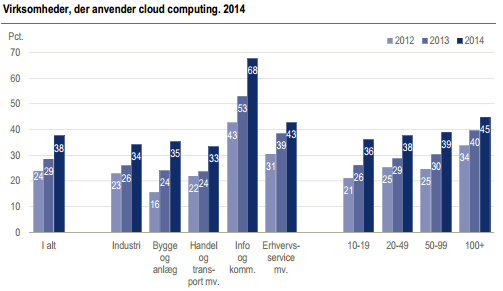
\includegraphics[width=1\textwidth]{figures/virksomhederderanvendercc.png}
    \caption{Statistik over virksomheder, som benytter cloud computing \citep{itvirk}.} 
    \label{fig:virksomcc}
\end{figure} \\

På figur \ref{fig:distcc} vises det, at over halvdelen \todo{kilde på figurer}af virksomhederne, bruger cloud computing til ting som filhåndtering og database brug, samt e-mail som også påtager næsten to tredjedele af alt cloud computing brug i virksomheder
. Yderligere vises det at over en tredjedel benytter det til infrastruktur, kundedata, økonomi mm. Cloud computing har den fordel, at det er allestedsnærværende. Uanset hvor en medarbejder befinder sig, enten på arbejde eller derhjemme, er der mulighed for at arbejde. I toget, derhjemme eller til møde, det er altid muligt at tilgå sine dokumenter, e-mails, applikationer osv.\todo{Følg den nu til dørs, Daniel - Uddyb!!! Færdiggør. Overgang til arejdsmiljø}
\begin{figure}
    \centering
    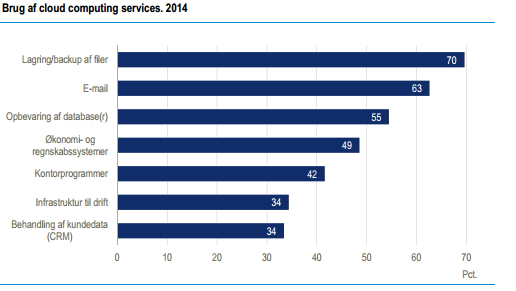
\includegraphics[width=1\textwidth]{figures/brugafccservices.png}
    \caption{Statistik over distribution af Cloud Computing brug \citep{itvirk}}
    \label{fig:distcc}
\end{figure}


%\section{Hvorfor mindre virksomheder ikke udvider}
%Der eksisterer en del mindre virksomheder indenfor byggebranchen, mange af dem vælger ikke at blive større, når håndværkermesteren indtjener det han gerne vil. Udover det virker administrationen for mange af de små virksomheder som uoverskuelig. De vælger ikke at udvide pga. manglende overskuelighed med hensyn til administration. Flere af dem frygter at miste overblikket over deres administration, hvis de udvider deres virksomhed og ansætter flere. I stedet vælger de at beholde deres størrelse, som en virksomhed på én til fire personer %\citep{SmaaFirmaerOrker}.
%I 2012 blev der indført en ny lov, som skræmte små virksomheder yderligere fra at udvide. Denne lov ville give virksomheder, som ikke havde administrationen i orden, bøder.\todo{Skal der bare stå bøder eller skal det omformuleres?} Denne lov rammer især de små virksomheder %\citep{Nyeadmboder}.
%Et eksempel på en type virksomhed, som ikke udvider, er håndværkervirksomheder. Tre ud af fire af disse virksomheder har kun én til fire ansatte. Dette skyldes som nævnt før, at de frygter administrationen af flere ansatte end dem de allerede har. De fleste af disse virksomheder er ofte ejet af en dygtig håndværker, hvor administration ikke er en del af personens %kompetencer \citep{SmaaFirmaerOrker}. \todo{Afsnittet skal generelt kigges på}


\section{Arbejdsmiljø}

\todo{Ikke start citat, hvem siger dette? Hvorfor er det vigtigt?}\textit{Arbejdsmiljø er et samspil af de relationer, påvirkninger og vilkår, som mennesket arbejder under. Det er også den tekniske og sociale udvikling af arbejdspladsen, som kan bidrage til det enkelte menneskes sikkerhed på kort sigt samt til menneskets fysiske og psykiske sundhed på længere sigt.} \citep{Arbejdsmiljoe}.
Et arbejdsmiljø kan have mange forskellige påvirkninger på arbejderen. Eksempler på disse kan være: 
\begin{itemize}
    \item {\textbf{Psykisk påvirkning} \citep{Arbejdsmiljoe_psykisk}}
    \begin{itemize}
    \item {\textbf{Stress}: At arbejde  kan være stressende, og dette kan have indvirkning på både arbejderen og arbejdsmiljøet. Stress kan f.eks. give hukommelsesbesvær, koncentrationsbesvær og nedsat humør. Disse faktorer kan både påvirke arbejderens arbejdsproces og arbejderens arbejdsomgivelser \citep{Arbejdsmiljoe_stress}.}
    \end{itemize}
    \item {\textbf{Fysisk påvirkning} \citep{Arbejdsmiljoe_fysisk}}
    \begin{itemize}
    \item {\textbf{Slid}: Et arbejde kan være fysiskt hårdt på mange måder. Dårlige muse anordninger til computerbrug kan f.eks. resultere i skader i håndled \citep{Arbejdsmiljoe_fysisk}.}
    \item {\textbf{Støj}: En larmende arbejdsplads kan også have stor indvirkning på arbejderens hørelse, i form af fysiske høreskader, men er også en faktor til psykisk stress \citep{Arbejdsmiljoe_stoej}.}
    \item {\textbf{Klima}: Aspekter som for høj eller for lav temperatur(højere end 25 grader, lavere end 20 grader), og et indelukket eller forurenet klima, kan have fysisk påvirkning på medarbejderen i form af f.eks. tørre øjne, træthed og hovedpine \citep{Arbejdsmiljoe_indeklima}.}\\
    \end{itemize}
\end{itemize}

\noindent Mangel på IT administration kan have stor negativ påvirkning på en arbejdsplads, og skabe et ineffektivt arbejdsmiljø. Denne negative påvirkning sker når der er mangel på effektiv IT administration f.eks. over-krævende- og uflexible arbejdsplaner, hvilket kan resultere i stress hos den enkelte medarbejder \citep{Cambridge2011}.\todo{Dette stykke skal placeres anderledes. Det skal muligvis skrive bedre sammen eller rykkes længere op}

\subsection{Vagtplanens indflydelse på arbejdsmiljø}
For at forebygge konsekvenserne af et dårligt arbejdsmiljø, er en struktureret eller fleksibel vagtplan en mulighed. En fleksibel vagtplan, hvor medarbejderen er med til at vælge sine vagter, vil udover at skabe en større medarbejdertilfredshed også ansvarliggøre medarbejderen. En fleksibel vagtplan vil sikre et bedre arbejdsmiljø, ved at skabe større fleksibilitet mellem arbejde og privatliv. Det øgede ansvar giver også medarbejderen en forståelse for arbejdsplanlægningen og dermed skabe et større engagement, i at få arbejdsplanen til at gå op. Samtidig vil vagtplanlæggeren få mere tid til andet arbejde som f.eks. kvalitetssikring.
Undersøgelser viser også, at gode og fleksible arbejdstider er fastholdelses potentiale for medarbejderne, hvilket vil sige at kontinuiteten opretholdes. 
Det næste afsnit tager udgangspunkt i artiklen: \textit{Ny fleksibel arbejdstid gav mere arbejdsglæde}
\citep{Thomse2014}.
\\
På et plejehjem i år 2010 blev der implementeret et IT-system, hvor medarbejderne selv skulle vælge sine vagter. Ifølge artiklen blev IT-systemet indført fordi \textit{Baggrunden var, at man gerne vil forebygge overbelastning af de stadig færre, der vælger at arbejde i sektoren og dermed også både fastholde dem i jobbet og rekruttere nye.}\todo{Omskriv} IT-systemet har givet medarbejderne mere frihed, fordi at muligheden for selv at vælge vagter, gør det lettere at tilpasse sig. Systemet virker ved at medarbejderne starter i en ønske fase, hvor de vælger de tider og dage de helst vil arbejde. Herefter bliver ønskerne puslet sammen i fællesskab, sådan at der altid er et tilstrækkeligt antal medarbejdere på arbejdet. Plejehjemmet udmelder at i denne sammenhæng, kan det være fornuftigt at have en blanding af medarbejdere der har, og ikke har børn. Denne flexible IT løsning reducerer også de mistænkelige sygedage (dage hvor man betvivler folks sygedom), fordi at medarbejderne selv fik mulighed for at vælge, hvilke dage de ville have fri. Den generelle stemning på arbejdspladsen er også blevet væsentligt bedre, da medarbejderne selv har valgt deres vagter, hvilket gør det svært at være utilfreds med arbejdstiderne. 
IT-systemet har derimod ikke kun været godt. I starten forholdte nogle af medarbejderne sig konservativt til løsningen og var tilfredse med vagtsystemet som de havde før. Efterhånden begyndte næsten alle dog at kunne se fordelene ved det nye IT-system. 

\section{Interessentanalyse}
\textbf{Hvad skal afsnittet indeholde?}
\begin{itemize}
\item{Analysen skal simulere at vi er et IT firma der laver et produkt som skal implementeres i en virksomhed}

\end{itemize}
\todo {Skal finde interessenterne for et problem}
Interessentanalyse bruges til at undersøge et problems interessenter og hvilke personer der har interessen for løsningen af dette problem, samt hvilken indflydelse de har på vigtige detaljer i løsningen. Derfor er denne analysemodel nyttig til at identificere de vigtigste interessenter, sådan at der tages forbehold for interessernes ønsker og eventuelle parter, som kunne ønske at have en dårlig indflydelse på produktet. Efter at interessenterne er identificeret gennem brainstorming, bliver de placeres i et Indflydelse-Medvirken matrix, som deler interessenterne i fire kategorier. En generel model af matrixen kan ses på figur []. Interessenter placeret i det øverste venstre hjørne hører under gruppen \textit{Gidslerne}. Det er interessenter som har lille indflydelse på projektets udformning, men alligevel er deres samarbejde nødvendig hvis processen skal blive en succes. Det er ofte personer der benytter produktet, der befinder sig i denne kvadrant. Derfor er det medarbejderne placeret her da de benytter sig af en vagtplansløsning, men ikke selv har en indflydelse på hvordan produktet bliver udformet. De benytter sig blot af løsningen. Nederst til venstre er de eksterne ressourcepersoner. Dette er interessenter som ikke bidrager med en aktiv medvirken, eller har indflydelse på produktet og er derfor ofte interessenter udenfor firmaet.  Derfor er andre virksomheder og kunderne placeret i denne kvadrant. De har ikke en direkte indflydelse på udfaldet af produktet og har heller ikke nogen indflydelse på hvordan produktet bliver udformet. Øverste til højre er ressourcepersonerne. Denne gruppe består af personer som har stor indflydelse og medvirken i projektet. De er ofte personer som har erfaringer med kravene til det nye system, samt hvordan dette skal implementeres. Derfor placeres arbejdsplanlæggerne her, da det er dem som har erfaring med hvordan firmaet normal lægger deres arbejdsplan og hvilke funktioner et program skal have, for at forbedre den hidtidige procedure. Den nederste højre kvadrant er de grå eminencer, som repræsenterer de personer som har stor indflydelse på produktet, men som ikke deltager aktivt i alle projektets detaljer. Chefer er placeret i dette felt, da de kan godkende eller afslå vigtige beslutninger omkring produktet, men samtidigt ikke medvirker aktivt i alle beslutninger. De kan dog vælge at gribe ind, hvis dette bliver nødvendigt.\\

\begin{figure}
    \centering
    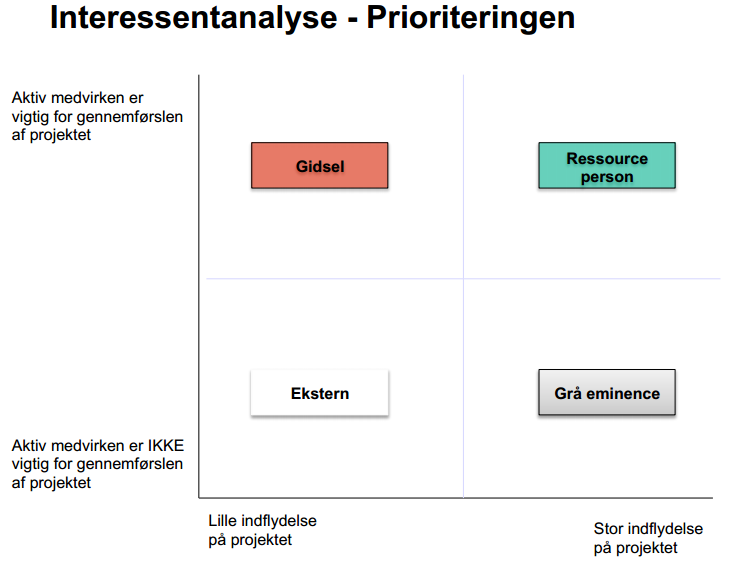
\includegraphics[width=1\textwidth]{figures/Udklip.PNG}
    \caption{Påvirkning og Indflydelse Matrix \citep{Holgaard2014}.} 
    \label{fig:PåvirkInflydMat}
\end{figure}

\subsection{Interessenter}
\textbf{Medarbejdere:}
Medarbejdere er interesseret i slutresultatet af projektet grundet, at de kommer til at benytte produktet i forbindelse med deres arbejde. Deres samarbejde er vigtig for gennemførelsen af projektet, da implementeringen afhænger af medarbejdernes samarbejdsvillighed. Selvom deres deltagelse er vigtig, har de ikke nogen indflydelse på projektets udformning, da det oftest vil være en chef, som står for arbejdsplanlægningen og dermed bruger de blot den gennemarbejdede arbejdsplan. Medarbejdernes holdninger  til projektet kan variere alt efter hvilken erfaring de har med det nuværende system. Det kan f.eks. være problematisk at skulle sættes ind i et nyt system, hvis de lige har lært at bruge det nuværende. Dog kan det også være at projektet tilvejebringer en bedre måde for dem at håndtere deres arbejdsplan hvorved de får mere overblik over deres arbejdstider.\\

\noindent\textbf{Chef:}
Chefer og ledelsen har stor interesse i projektet, da det primært er dem som holder overblik over medarbejderne og sørger for at de kommer til tiden. Derfor kunne de være interesserede i et struktureret skema, til at holde overblik over medarbejderne. Bedre struktur kan også gøre det muligt for chefen at holde styr på hvor meget den individuelle medarbejder arbejder, sådan at reglerne om arbejdstid overholdes.\\

\noindent\textbf{Arbejdsplanlægger:}
Arbejds planlæggeren er vigtig for udviklingsprocessen, da det er denne person, som har stor erfaring med det nuværende system og kender behovene for arbejdsplanlægningen. Herved kan denne person forklare de krav og behov som arbejdsplanlægningen kræver. På dette grundlag, har arbejds planlæggeren en stor indflydelse på projektet. Yderligere er det vigtigt at personen aktivt medvirker i projektet for at dette bliver en succes. \\


\noindent\textbf{IT-leverandør:}
IT-leverandøren er det firma som sælger eller eksporterer et IT-produkt til virksomheden. De sælger produkter som computere, telefoner eller lignende, som skal hjælpe virksomheden med dens administration.
IT-leverandøren er i den Ekstern gruppe, da de ikke har stor indflydelse på projektet og ikke har en vigtig medvirken i gennemførelsen af projektet. De søger dog for udstyr som kan bruges af virksomheden efter produktet er blevet udviklet.\\

\noindent\textbf{Kunderne:}
Kunderne for firmaet er også en interessent da de modtager den service som firmaet tilbyder og er derfor direkte påvirkede af firmaets effektivitet. Kunderne er brugere af firmaet men de har ikke noget indflydelse eller medvirken på projektet. De bliver indirekte påvirket af projektet, hvilket er grunden til at de ikke har nogen indflydelse på udformningen af projektet.
\todo{Staten er interessant hvis sygefravær og stress kan mindskes}\\

\section{Det kvalitative interview}\todo{Skal sættes op før teknologivurderingen da de bidrager med gode og dårlige sider af programmerne som er en del af teknologivurderingen}
Det kvalitative forskningsinterview forsøger at forstå verden fra informantens synspunkt, herunder meninger og holdninger. Viden i forskningsinterviewet skabes i interaktionen mellem interviewer og informant. Interview er valgt frem for et spørgeskema, da den viden man får ved et interview, ikke nødvendigvis ville opstå i en spørgeskemaundersøgelse. Interview giver informanten mulighed for at fordybe sig i og udforske egne oplevelser og meninger. Den viden der opnås ved et interview, er socialt konstrueret, da det ikke bare er en dataindsamling, men at der skabes data gennem den førnævnte interaktion \citep{kvale2009}.
\\\\
Ved hjælp af interessentanalysen, er det blevet klargjort, hvilke personer der kunne være interesserede i en løsning. Ved interviewene stræbes der efter at opnå en viden omkring hvilke problemer der er ved nuværende løsninger, samt krav til fremtidige løsninger. Interviewet blev herefter brugt til at skabe indsigt indenfor emnet. Spørgsmålene blev lavet på baggrund af nogle emner der skulle belyses. Udfra disse emner, blev nogle korte og åbne spørgsmål lavet, for at sikre, at den viden der opstod blev reflekteret over. Dette ville ikke være muligt med f.eks. ledende spørgsmål, hvor man risikerer at påvirke informanten i en bestemt retning. Ved hjælp af svarene fra interviewene blev det gjort klart, hvilke problemer der var med de nuværende systemer, samt positive sider heraf. Udfra disse data kunne en foreløbig kravspecifikation dannes.
\\
\subsection{Sammendrag af interviews}
\textbf{Home, Aalborg} \\
Hos Home benytter de sig af en manuel løsning i form af en kalender der synkroniseres med Outlook. Hver tredje bliver der lavet en ny vagtplan for medarbejderne. De kører sammen med Hasseris afdelingen, men har ingen umiddelbar indflydelse på andres vagtplaner end deres egen. Når der skal byttes vagter bliver dette gjort internt, samt hvis en person er syg, bliver dette også ordnet internt. Da de også er fastansatte, gør dette også, at der ikke skal byttes så ofte.
Da de har fast struktureret vagtplan, kan der ikke uddrages så meget her angående fleksible vagtplaner. En vigtig feature er dog, at vagtplanen kan synkroniseres med andre kalendere.
En direkte transskribering kan findes i XXX.\todo{Få ordnet kilde}\\\\
\textbf{KIWI, Aalborg}\\
I KIWI benytter de sig af et et vagtplanlægningssystem der hedder Staffweb, hvor medarbejderne kan tilgå vagterne via internettet, mens vagtplanlæggeren kan styre planen via et program på hans computer. Medarbejderne kan med dette system, gå ind og frigive deres vagter, hvis ikke de kan arbejde den pågældende dag.
Af mangler bliver der nævnt, at der mangler en funktion, der kan udskifte en hel persons vagter, hvis vedkommende stopper, sådan at en ny kan overtage.
Som de selv beskriver det så; “..I forhold til før hvor vi havde det på papiret, der er det nemmere, fordi enhver har ikke undskyldningen med, min vagtplan er blevet væk, fordi man kan altid bare gå ind på nettet..”.
En direkte transskribering kan findes i XXX.\todo{Og kilde her}


\section{Teknologivurdering}
\todo{Hvad indeholder en teknologivurdering og hvordan er jeres opbygget.}
I projektet er der blevet undersøgt tre systemer, der hjælper med vagtplanlægning; Tamigo, Planday og Lectio. Denne undersøgelse bestod af at identificere hvad nuværende løsninger er i stand til, samt at bestemme fordele og ulemper ved disse løsninger. Udfra disse informationer kan der bestemmes foreløbige krav til en mulig løsning til projektet.
\todo {Efter overskrift - hvad indeholder tekno vurdering og hvordan er rapport opbygget}
\subsection{Tamigo}
Tamigo er et online vagtplanlægningsværktøj som har flere forskellige funktioner. Disse funktioner tillader bl.a. administratoren at planlægge effektivt efter de gældende timeregler. Deltidsarbejderne har desuden mulighed for at bytte deres vagter og anmode om fridage online sådan at arbejdsgiveren kan bevare overblikket.\\

\textbf{Fordele: }
\begin{itemize}
\item {Tæller medarbejdernes timer og advarer arbejdsgiveren hvis antallet overskrides eller undermineres.}
\item {Vagtbytnings funktion som har indbygget dokumentation af ændringerne.}
\item {Apps til smartphones som tillader medarbejderne at se planen online.}
\item {Programmet og appen indeholder en telefonliste over medarbejderne som gør kontakt mellem arbejder og arbejdsgiver nemmere.}\\
\end{itemize}

\textbf{Ulemper: }
\begin{itemize}
\item {Kan ikke ses uden internetforbindelse.}
\item {Kan virke uoverskuelig hvis ikke man er blevet sat ind i systemet \citep{Tamigo, Trustpilot}.}
\end{itemize}


\todo{interview en fra en tamigo butik sådan at vi har noget info at skrive på}

\subsection{Planday}
Planday er en online vagtplan udbyder, som kan tilgås igennem platforme som f.eks. computere, tablets og mobiltelefoner. Planday har mange funktioner. Eksempler på disse er:
\begin{itemize}
\item {\textbf{Sygemelding:} Man kan melde sig syg online. Derefter kan vagtplanlæggeren se at vedkommende er syg. Vagtplanlæggeren kan herved trykke på den syges vagt og se hvilke medarbejdere der er ledige med samme kvalifikationer som den syge, og derefter vælge medarbejdere. De valgte medarbejdere vil så få en besked eller mail, om vedkommende gerne vil overtage vagten.}
\item {\textbf{Forum:} Planday tilbyder et forum. I dette forum kan chefen og alle virksomhedens medarbejdere kommunikere med hinanden, f.eks. med henblik på at bytte vagter, ferieplanlægning osv.}
\item {\textbf{Oversigt over timeantal:} Der kan ses hvor mange timer der er arbejdet, og hvor meget løn der er berettiget.}
\item {\textbf{Kundeservice:} Planday er behjælpelige når der opstår problemer hos brugeren. Når de får dårlige anmeldelser, så skriver de en hjælpende kommentar til anmeldelsen.} 
\end{itemize} 
\citep{DanskInternetHandel, Simonsen2014, Planday}.\\\\

Ud fra brugeranmeldelser lavet omkring Planday, er der også fundet negative aspekter ved Planday. Eksempler på disse er:
\begin{itemize}
\item {\textbf{Effektivitet:} Plandays browserversion er mere effektiv end appen.} 
\item {\textbf{Utilregnelig:} Appen crasher nogle gange ved opstart.}
\item {\textbf{Information:} Den kan heller ikke altid vise de beskeder man modtaget og man kan ikke se om ens ferie er godkendt.} 
\item {\textbf{Tilgængelighed:} Kan ikke tilgås uden en online platform}
\end{itemize}
\todo{omskrives}\citep{Play}. \\

\subsection{Lectio}
\todo {Er det relevant?}
Lectio er et planlægningsværktøj som primært bliver brugt på gymnasier mellem lærere og elever. Servicen gør det muligt for lærere at lave et tilrettelagt skema som eleverne kan tjekke online. Udover det kan lærerne også dynamisk aflyse og flytte lektioner. Lectios anden primære funktion gør det muligt for den enkelte elev at uploade opgaver til Lectios servere hvor der bliver holdt styr på elevens totale afleveringsprocent samt fysisk fravær \citep{Macom}.





\section{Problemafgrænsning}

\section{Problemformulering}